\section{Principal Component Analysis}
%
%
\subsection{Principal Component Analysis, the classical statistical tool}
The Principal Component Analysis (PCA) is a statistical technique for data dimensionality reduction. It looks for the so-called {\em Principal Components} (PCs for short), which are vectors that form an orthonormal 	basis for $\mathbb{R}^\traceLength$. Such PCs are computed, via singular value decomposition, as the eigenvectors of the empirical covariance matrix of data: given a set of data $(\sss[]{i})_{i=1,\dots,\numTraces[]}$ the empirical covariance matrix is given by
\begin{equation}\label{eq:covmat}
\covmat = \frac{1}{\numTraces[]} \sum_{i=1}^{\numTraces[]}(\sss[]{i} - \mmmX)(\sss[]{i} - \mmmX)^T \mbox{ ,}
\end{equation}
 where $\mmmX$ is the empirical mean of data. Let us denote $\AAlpha_1, \dots, \AAlpha_r$ the eigenvectors of such a matrix (where $r$ denotes its rank) and $\lambda_1, \dots, \lambda_r$  the corresponding eigenvalues, sorted in decreasing order. It can be shown that $\lambda_i$, for each $i$, equals the empirical variance of data projected onto the corresponding PC $\AAlpha_i$. Since the variability of data is associated to the amount of information data hold, transforming data over the basis provided by the PCs allows a dimensionality reduction that minimizes the loss of information: that is keeping only the leading $\newTraceLength$ PCs and projecting data on the $\newTraceLength$-dimensional space they span.\\

\subsection{Principal Component Analysis, the {\em Class-Oriented Version}}
In SCA context, the useful information part contained in data is the one that allows to discriminate observations linked to different intermediate computations. Let us denote by $\sensRandVar = \targetFunction(\randPlaintext,\randKey)$ the target intermediate variable, that depends on both a secret variable $\randKey$ and on a public known one $\randPlaintext$, and that takes values $\sensVar \in \sensVarSet$. The attack will be the more efficacious the more the extractor used by the attacker amplifies the distinguishability between traces associated to different intermediate values $\sensVar$.\\
Since during the profiling phase the attacker knows the value $\sensVar$ of the sensitive variable handled during each acquisition, she can assign to each profiling trace the {\em class} $\sensVar$ (in analogy with the pattern recognition terminology), obtaining the labelled profiling set $(\sss{i})_{i=1,\dots,\numTraces}$, where $\numTraces$ is the number of traces belonging to the class $\sensVar$. This knowledge is very useful to construct a good class-distinguishing extractor, but the classical PCA does not exploit it. For this reason in SCA literature a {\em class-oriented} version of PCA is often used instead of the classical one. This version  consists in applying PCA to the set of class-average traces $(\mmmXclass)_{\sensVar \in \sensVarSet}$, instead of to the whole set of traces, where $\mmmXclass$ is the empirical mean of traces belonging to the same class $\sensVar$: this implies that the empirical covariance matrix will be computed using only the $\lvert \sensVarSet \rvert$ average traces. Equivalently, in case of equilibrated acquisitions ($\numTraces$ constant for each class $\sensVar$), it consists in using instead of the covariance matrix $\covmat$ of data, the so-called {\em between-class} or inter-class {\em scatter matrix}, given by
\begin{equation}\label{eq:SB}
\SB = \sum_{\sensVar\in\sensVarSet}\numTraces(\mmmXclass-\mmmX)(\mmmXclass-\mmmX)^T \mbox{ .}
\end{equation}
Remark that $\SB$ coincides, up to a multiplicative factor, to the covariance matrix obtained using the class-averaged traces.

\subsection{Computational Trick to Avoid the Computation of Big Covariance Matrices}
Performing PCA (or LDA, as we will see in next section), always asks to compute the eigenvectors of some symmetric matrix $\covmat$, obtained by the multiplication of a constant, a matrix $\measuresMatrix$ (e.g. for class-oriented PCA $\measuresMatrix = [\sqrt{\numTraces[\sensVar_1]}(\mmmXclass[\sensVar_1]-\mmmX),\sqrt{\numTraces[\sensVar_2]}(\mmmXclass[\sensVar_2]-\mmmX), \dots ]$), and its transposed . Let $\measuresMatrix$ have dimension $\traceLength\times\numTraces[]$, and suppose $\numTraces[]\ll \traceLength$, as it might be the case, e.g. in class-oriented PCA version it is often the case, since $\numTraces[]=\lvert \sensRandVar \rvert$. Thus, the matrix $\covmat=\measuresMatrix\measuresMatrix^T$ is far from being a full-rank matrix: $\mathrm{rank}(\covmat)\leq \numTraces[]$. For this reason, we can obtain at most $\numTraces[]$ eigenvectors; moreover, often rows of $\measuresMatrix$ are linearly dependent, as in our example, since they are forced to have zero mean, so actually the rank of $\covmat$ is strictly less than $\numTraces[]$ and we expect can obtain at most $\numTraces[]-1$ eigenvectors.\\
A practical problem in case of high-dimensional data, i.e. $\traceLength$ big, is represented by the computation and the storage of the $\traceLength\times\traceLength$ matrix $\covmat$. This problem can be circumvented exploiting the following lemma coming from linear algebra:
\begin{lemma}
For any $\traceLength\times\numTraces[]$ matrix $\measuresMatrix$, mapping $\xxx\mapsto \measuresMatrix \xxx$ is a one-to-one mapping that maps eigenvectors of  $\measuresMatrix^T\measuresMatrix$ ($\numTraces[]\times\numTraces[]$)    onto those of   $\measuresMatrix\measuresMatrix^T$ ($\traceLength\times\traceLength$).
\end{lemma}
%
This lemma allows to compute and store the $\numTraces[]\times\numTraces[]$ matrix $\tilde{\covmat} = \frac{1}{\numTraces[]}\measuresMatrix^T\measuresMatrix$, compute its $\numTraces[]\times 1$ eigenvectors $\BBeta_i$ and eigenvalues $\lambda_i$, convert them into eigenvectors of $\covmat$: $\AAlpha_i = \measuresMatrix\BBeta_i$. It is not guaranteed that eigenvectors $\AAlpha$ obtained in this way have norm equal to 1. This is why a normalization step should follow if we aim to obtain an orthonormal set of eigenvectors.


\subsection{The Open Question: Choosing the Components to Keep?}
The introduction of PCA method (either in its classical or class-oriented version) in SCA context has opened some important questions: how many principal components are sufficient/necessary to efficiently reduce the trace size without losing important discriminative information? And which of such components are those that most point out the effective vulnerable time samples that most leak information?\\
Until now, an answer to the first question were given, linked to the concept of {\em explained variance} (or {\em explained global variance}, EGV for short) of a PC $\AAlpha_i$:
\begin{equation}\label{eq:EGV}
\mathrm{EGV}(\AAlpha_i) =  \frac{\lambda_i}{\sum_{j=1}^r\lambda_j} \mbox{ ,}
\end{equation}
where $r$ is the rank of the covariance matrix $\covmat$. The EGV is the variance of data projected over the $i$-th PC (which equals $\lambda_i$) divided by the total variance of original data (given by the trace of the covariance matrix $\covmat$). The sum of all the PCs EGV is equal to $1$; that is why this quantity is often multiplied by $100$ and expressed as percentage.
The notion of EGV offers a quite natural answer to the first question above: the idea is to fix a wished {\em Cumulative Explained Variance} $\beta$ and to keep $\newTraceLength$ PCs, where $\newTraceLength$ is the minimum integer such that
\begin{equation}
\mbox{EGV}(\AAlpha_1) +\mbox{EGV}(\AAlpha_2) + \dots +\mbox{EGV}(\AAlpha_\newTraceLength) \geq \beta \mbox{ .}
\end{equation}
Nevertheless this method takes for granted that the optimal way to chose PCs is in their natural order, from the first to the $i$-th, answering trivially to our second question. But in SCA this assumption is not confirmed: in some works, researchers remarked that in SCA context the first components sometimes contain more noise than information and it is worth discarding them. For the sake of providing you a fast example of this behaviour on public accessible traces, we applied a class-oriented PCA on 3000 traces downloaded by the DPA contest v4 trace set; we focused over a small 1000-dimensional window in which, in complete knowledge about masks and other countermeasures, information about the first round first byte Sbox output leaks. Figure~(\ref{fig:DPAcontest}) shows the first and the sixth PCs. We remark that the first components indicates that one can attend a high variance in data exploiting the regularity of the traces, given by the clock signal, while the sixth is the first one in the order the focus on the actually leaking point.

\begin{figure}
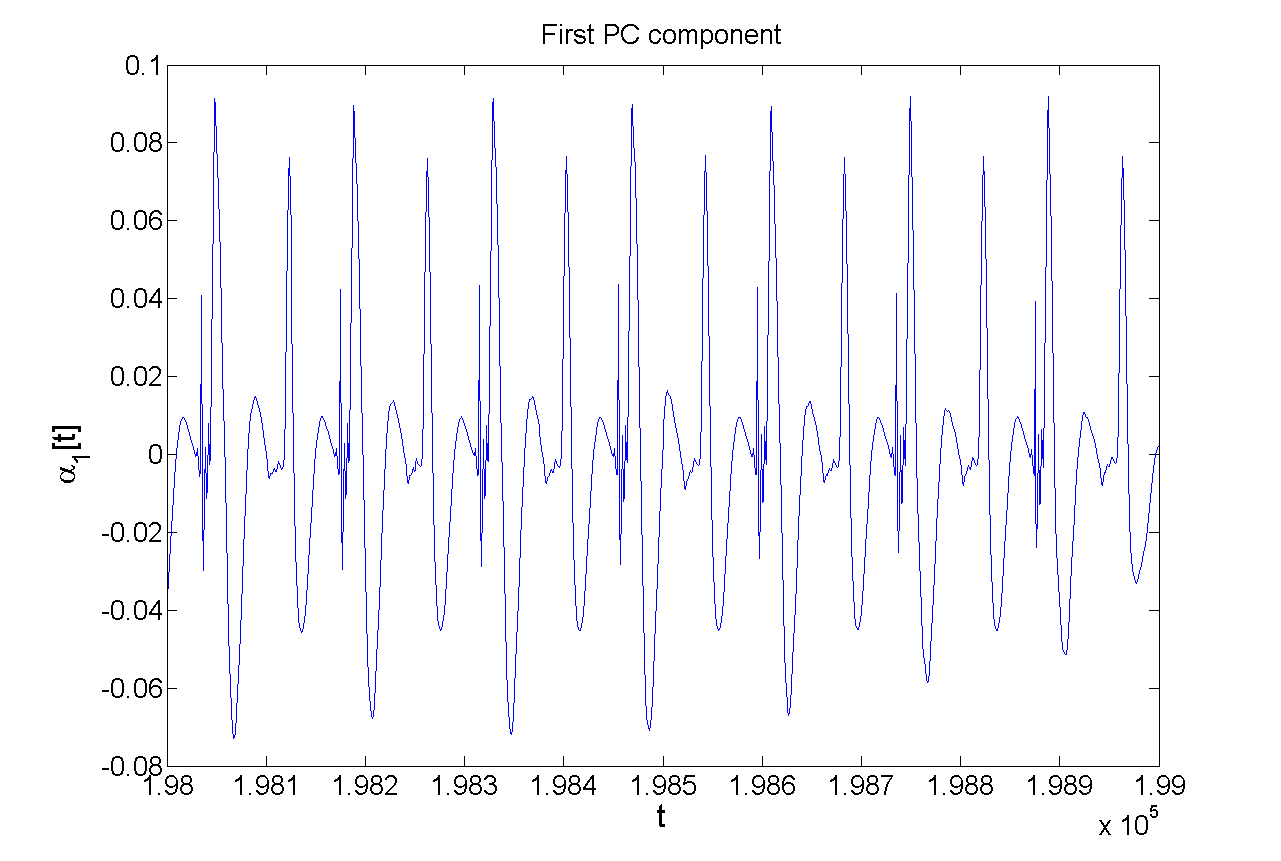
\includegraphics[width=.5\textwidth]{figures/PC_1_10000_198001_199000.png} 
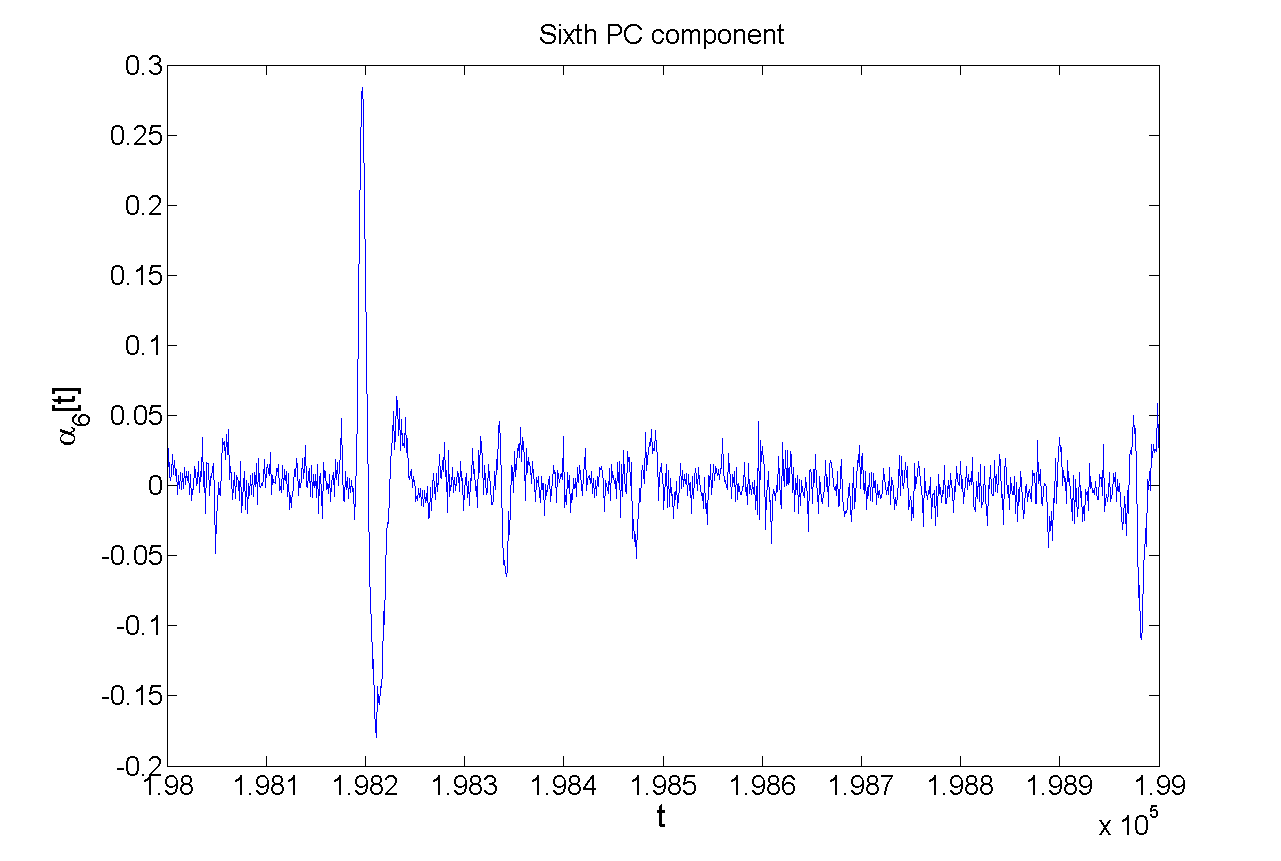
\includegraphics[width=.5\textwidth]{figures/PC_6_10000_198001_199000.png} 
\caption{First and sixth PCs in DPA contest v4 trace set}\label{fig:DPAcontest}
\end{figure}
To the best of our knowledge, until now only one method was proposed to automatically chose PCs to keep in order to perform an efficacious SCA \cite{SCAclassProbl}, and was based on the same assumption we find reasonable to consider:
\begin{assumption}\label{assum:local}
The leaking side-channel information is localised in few points of the acquired trace.
\end{assumption}
Under this assumption, in \cite{SCAclassProbl} a measure to evaluate the eigenvectors' {\em localization} is proposed, called {\em Inverse Participation Ratio} (IPR)
\begin{equation}
\mathrm{IPR}(\AAlpha_i) = \sum_{t=1}^\traceLength \AAlpha_i[t]^4 \mbox{ ,}
\end{equation}
and it is suggested to collect PCs to be kept for SCA purpose in decreasing order with respect to such a measure.\\
We remark that this measure completely discards the information given by the eigenvalues of the PCs. We will compare this selection method with the standard one, that we will denote by EGV, and with a new one that we propose in next section.

%
\subsection{The Explained Local Variance Selection Method} 
The method we propose is based on a compromise between the variance provided by each PC and the number of time samples necessary to achieve a consistent part of such a variance. To this purpose let us introduce the concept of {\em Explained Local Variance} (ELV, with this acronym we will also refer to the selection method): thinking to observations ${\sss[]{}}^\mathrm{T}$, or class-averages ${\mmmX}^\mathrm{T}$ in class-oriented PCA case, as realizations of a random variable $\XXX$, we have that $\lambda_i$ is an estimator for the variance of the random variable $\XXX\AAlpha_i$. Developing, we obtain
\begin{align}\label{eq:ELV}
\lambda_i =& \hat{\mathrm{var}}(\sum_{t_1=1}^D \XXX[i]\AAlpha_i[t_1]) = \sum_{t_1=1}^D\sum_{t_2=1}^D \hat{\mathrm{cov}}(\XXX[t_1]\AAlpha_i[t_1], \XXX[t_2]\AAlpha_i[t_2])=\\
=& \sum_{t_1=1}^D \AAlpha_i[t_1]\sum_{t_2=1}^D\AAlpha_i[t_2]\hat{\mathrm{cov}}(\XXX[t_1], \XXX[t_2])= \sum_{t_1=1}^D \AAlpha_i[t_1]\cdot \covmat_{t_1} \AAlpha_i=  \\
=& \sum_{t_1=1}^D \AAlpha_i[t_1]\cdot \lambda_i\AAlpha_i[t_1]= \sum_{t_1=1}^D  \lambda_i \AAlpha_i[t_1]^2
\end{align}
where $\covmat_{t_1}$ indicates the $t_1$-th row of $\covmat$ and the last line is justified by the fact that $\AAlpha_i$ is an eigenvector of $\covmat$, with $\lambda_i$ its corresponding eigenvalue. The result of this computation is quite obvious, since $\parallel \AAlpha_i\parallel=1$, but it evidences the contribute of each time sample in the information held by the PC. This makes us introduce the following definition:
\begin{definition}
The {\em Explained Local Variance} of a PC $\AAlpha_i$ in a sample $j$, is defined by
\begin{equation}
\mathrm{ELV}(i,t) = \frac{\lambda_i \AAlpha_i[t]^2}{\sum_{j=1}^r\lambda_j} = \mathrm{EGV}(i) \AAlpha_i[t]^2  \mbox{ .}
\end{equation}
\end{definition}
The sum over all the trace samples ELVs of a PC equals the EGV of the considered PC.\\
The ELV selection method, in analogy with the EGV one, consists in fixing a a threshold value $\beta$ for the wished {\em Cumulative Explained Local Variance} and construct the set 
\begin{equation}
S = \{(i_1, t_1), \dots , (i_{\newTraceLength},t_{\newTraceLength})\} 
\end{equation}
where $\newTraceLength$ is the minimal integer such that
\begin{equation}
\mathrm{ELV}(i_1,t_1)+\dots +  \mathrm{ELV}(i_{\newTraceLength},t_{\newTraceLength})\geq \beta \mbox{ .}
\end{equation}
The rule to choose PCs to keep is then
\begin{equation}
\mbox{Keep } \AAlpha_i \Leftrightarrow \exists t \mbox{ such that } (i,t)\in S \mbox{; }
\end{equation}
moreover, we propose to only consider, among time samples of each chosen PC, those that hold a significant ELV. For this reason we suggest to consider new PCs $\tilde{\AAlpha}_i$, that we believe incorporate less noise, constructed as follows:

\begin{equation}
\tilde{\AAlpha}_i[t] = \begin{cases}
\AAlpha_i[j] \mbox{ if } (i,t)\in S\\
0 \mbox{ otherwise.}
\end{cases}
\end{equation}
%Moreover we define the {\em ELV vector} of a PC $\AAlpha_k$ as the vector $\vectorContribution = (\mathrm{ELV}(k,i))_{i=1..\traceLength}$.
%\end{definition}
%
%
%\subsubsection{{\em Cumulative Explained Local Variance} selection method}
%In this section we present how to select the most informative PCs and how to modify them in order to meaningfully obtain interesting PVs for side channels context.\\
%
%Let $r$ be the rank of the covariance matrix $\covmat$, i.e. the total number of PCs, $\AAlpha_1, \dots, \AAlpha_r$.\\
%Let $\coupleSet = \{1,\dots, r\}\times \{1,\dots,\traceLength\}$ and let us introduce a succession of index couples as
%
%\begin{equation}
%\begin{cases}
%(k_1, i_1) = \mathrm{argmax_{(k,i)\in \coupleSet}}\mathrm{ELV}(k,i)\\
%(k_j, i_j) = \mathrm{argmax_{(k,i)\in \coupleSet\smallsetminus \{(k_1,i_1),\dots,(k_{j-1}, i_{i-1})\}}}\mathrm{ELV}(k,i)\mbox{ .}
%\end{cases}
%\end{equation}
%
%Now fix 
%
%\begin{remark}
%Let $A$ be the matrix that contains the chosen $\tilde{\AAlpha}_k$ vectors as columns. The total variance $\sum diag(A^T\covmat A)$ will not attend the  $\beta$-th part of the initial variables variance, as it would be if eigenvectors $\AAlpha_k$ would have been kept unchanged, but will be lower than it. This is exactly because  vectors $\tilde{\AAlpha}_k$ are no more eigenvectors of $\covmat$. 
%\end{remark}
%
%
%\paragraph{A practical problem that might occur: linear dependent projected data}
%Since the proposed method suggests changing the PCs into new projecting vectors $\tilde{\AAlpha}_k$, the property of decorrelating principal variables is lost. On the contrary it might happen, especially if some $\tilde{\AAlpha}_k$ have only a few non-zero coefficients, that data are projected into new  perfectly correlated coordinates. That is a problem if, for example, the projected data are intended to be used to construct templates for a template attack: the covariance matrix of a random vector with two or more perfectly correlated components is singular, thus, non-invertible, and if templates have non-invertible covariance matrices the template attack is impracticable. \\
%Let $A = [\AAlpha_1, \dots , \AAlpha_\newTraceLength]$ be the matrix containing as columns the projecting components chosen via \emph{Cumulative ELV method}. The problem just described arises whenever such components present a linear dependency, i.e. the matrix $A$ has not maximal rank. This means that one or more components just create new projected variables that are linear combinations of variables constructed by the other components. In practice one or more components do not add any information, and their suppression would not cause an effective lost of \emph{ELV}. That is why as a last passage of our method we propose to check that the projecting matrix has maximal rank $\newTraceLength$, and, if it has not, suppress from it the minimal number of columns that makes it attend its maximal rank. 
%
%
%
%
